% ----------------------------- CONCETTI AVANZATI ------------------------------------

\chapter{Concetti Avanzati}

% Argomenti di questo capitolo:

% unique pointers
% smart pointers
% shared pointer
% weak pointers
% friend functions
% e make unique

%TODO: Copy-and-Swap Idiom?
%TODO: Signal Handling? (magari in un capitolo sul multithreading)
%TODO: Prevent Object Copy?
%TODO: Command Line Arguments?

%TODO: tecniche per debuggare codice?
%TODO: Writing C++ code efficiently in Competitive Programming?

%TODO: 7 Advance C++ Concepts: RAII, Return Type Resolver, Type Erasure, CRTP, Virtual Constructor, SFINAE, Proxy.

%TODO: pointer to function?

% std uniform real distribution

% C++ 20: Concepts, ranges, coroutines, template parameter list, modules, ecc.. (non qui, ma in Le gemme della libreria degli Algoritmi)

%TODO: Dependency Injection
%TODO: std::static_pointer_cast
%TODO: std::enable_share_from_this
%TODO: allocate_shared
%TODO: Allocator
%TODO: std::bad_alloc

%TODO: std::clamp (non è chi sa che cosa di avanzato, comunque).
%TODO: normal_distribution

%TODO: magari aggiungere nel capitolo "basi del linguaggio": struct destructors che servono se allochi della memoria nelle struct, non se le usi, ma se allochi.

%TODO: xvalue?

%TODO: performance optimization, performance, optimization techniques?
%TODO: un esempio è usare ++i al posto di i++
%TODO: esempi: Premature Pessimization to avoid Premature Optimization.

% -------------------------- SECTION: INTRODUZIONE -----------------------------------

\section{Introduzione}

\textsf{\small In questo capitolo "finale" tratterò argomenti un po' più complessi o che almeno non mi verrebbe da mettere negli altri due capitoli precedenti.} \\

\textsf{\small Verranno trattati argomenti come gli smart pointers e quindi unique pointers, share pointers, weak pointers, le friend function, uniform real distribution e altri importanti concetti avanzati.} \\

% -------------------------- SECTION: FRIEND KEYWORD ---------------------------------

\newpage

\section{Friend Keyword}

\subsection{Friend Class}

\textsf{\small \textbf{Definizione: } La keyword \textbf{friend} è usata per accedere ai membri privati e protetti di una classe nella quale è dichiarata \textbf{friend}.} \\

\begin{lstlisting}
	#include <iostream>
	
	class A {
		public:
			A() { a = 0 };
			friend class B; // Classe amica.
			
		private:
			int a;
	};

	class B {
		public:
			void showA(A& x)
			{
				// Visto che B è un'amica di A, può accedere ai membri privati di A.
				std::cout << "A::a : " << x.a; 
			}
	};

	int main()
	{
		A a;
		B b;
		b.showA(); //Output: A::a : 0
		return 0;
	}
\end{lstlisting}

\subsection{Friend Function}

\textsf{\small \textbf{Definizione: } Come per le \textbf{classi friend}, una \textbf{funzione friend} ha accesso speciale ai membri privati e protetti.} \\

\textsf{\small Una \textbf{friend function} può essere: } \\

\begin{itemize}
	\item \textsf{\small Un membro di un'altra classe.}
	\item \textsf{\small Una funzione globale.}
\end{itemize}

\textsf{\small Alcuni importanti punti riguardo alle \textbf{friend} functions e classes: } \\

\begin{itemize}
	\item \textsf{\small Dovrebbero essere usate solo in maniera limitata. Troppe funzioni o classi \textbf{friend} diminuiscono l'encapsulazione.}
	\item \textsf{\small L'amicizia non è reciproca. Se la classe A è amica della classe B, allora B non è automaticamente amica di A.}
	\item \textsf{\small L'amicizia non è ereditata.}
	%\item \textsf{\small }
\end{itemize}

\begin{lstlisting}
	#include <iostream>
	
	class A {
		public:
			friend void printWidth( A a);
			void setWidth(double w);
			
		private:
			double width;
	};

	// Definizione della funzione membro di A.
	void A::setWidth(double w)
	{
		width = w;
	}

	// printWidth non è una funzione membra di nessuna classe.
	void printWidth( A a )
	{
		// Visto che la funzione printWidth è amica di A, può accedere direttamente a qualsiasi membro di A.
		std::cout << "Width di A: " << a.width << std::endl;
	}

	int main()
	{
		A a;
		
		a.setWidth(11.1);
		
		// Uso la funzione amica per stampare la width di a.
		printWidth( a ) ; //Output: Width di A: 11.1
		return 0;
	}
\end{lstlisting}

% -------------------------- SECTION: SMART POINTERS ---------------------------------

\newpage

\section{Smart Pointers}

\textsf{\small \textbf{Definizione: } Gli \textbf{smart pointers} (puntatori intelligenti) sono dei puntatori che, in più rispetto ai normali puntatori, sono in grado deallocare la memoria automaticamente, senza che il programmatore debba occuparsene ed evitando \emph{memory leak}.} \\

\subsection{Differenze con i puntatori normali}

\textsf{\small I \textbf{puntatori} servono per poter accedere a delle risorse che sono esterne al programma (alla memoria heap). Grazie ai puntatori saremo in grado di modificare direttamente la risorsa esterna, al posto di doverne fare una copia.} \\

\textsf{\small Il problema di questi puntatori è che se non deallocati correttamente potrebbero portare ad uno spreco della memoria heap, il che è un \emph{memory leak}.} \\

\begin{lstlisting}
	#include <iostream>
	
	class Rectangle {
		private:
			int width;
			int height;
	};

	void fun()
	{
		Rectangle* p = new Rectangle();
	}

	int main()
	{
		while(1)
		{
			fun();
		}
		//Output: Il problema è che quando la funzione fun termina, il puntatore p verrà distrutto come fosse una variabile locale, ma la memoria allocata non verrà deallocata, perché ci siamo scordati di usare \emph{delete p}; alla fine della funzione.
		
		// Ciò è un problema perché verrà sempre allocata altra memoria e mai deallocata, occupando spazio, sprecando memoria, il che è un \emph{memory leak}.
		
		// L'intera memoria heap potrebbe diventare inutile per questo motivo. 
		return 0;
	}
\end{lstlisting}

\textsf{\small Il problema è che quando la funzione fun termina, il puntatore p verrà distrutto come fosse una variabile locale, ma la memoria allocata non verrà deallocata, perché ci siamo scordati di usare \emph{delete p}; alla fine della funzione.} \\

\textsf{\small Ciò è un problema perché verrà sempre allocata altra memoria e mai deallocata, occupando spazio, sprecando memoria, il che è un \emph{memory leak}.} \\

\textsf{\small L'intera memoria heap potrebbe diventare inutile per questo motivo. } \break

\textsf{\small Uno \textbf{smart pointer} è un \emph{wrapper} (un wrapper è un'entità che ne encapsula un'altra; è del codice che letteralmente avvolge, incarta, impacchetta, confeziona dell'altro codice) su un puntatore con un'operatore \textbf{*} e \textbf{->} overloaded.} \\

\textsf{\small La memoria allocata dinamicamente verrebbe così automaticamente liberata.} \\

\begin{lstlisting}
	// Una generica classe Smart Pointer
	#include <iostream>
	
	template <class T>
	class SmartPointer {
		T *ptr;
		public:
			SmartPointer(T *ptr = NULL)
			{
				p = ptr;
			}
		
			~SmartPointer()
			{
				delete ptr;
			}
		
			T & operator * ()
			{
				return *ptr;
			}
		
			T * operator ->()
			{
				return ptr;
			}
	};

	int main()
	{
		SmartPointer<int> p(new int());
		*p = 22;
		std::cout << "Valore di *p: " << *p << std::endl; //Output: Valore di *p: 22
		return 0;
	}
\end{lstlisting}

%TODO: unique, share, weak, 
%TODO: std::make_unique vs std::unique_ptr
%TODO: std::make_shared

%TODO: problemi dei vecchi puntatori.

%TODO: std::static_pointer_cast
%TODO: std::enable_share_from_this
%TODO: allocate_shared
%TODO: Allocator
%TODO: std::bad_alloc
%TODO: auto_ptr (C++98)

%TODO: dynamic_pointer_cast
%TODO: const_pointer_cast

\subsection{unique pointers}

\textsf{\small \textbf{Definizione: } Gli \textbf{unique pointers} sono un tipo di \textbf{smart pointers} che memorizzano un solo puntatore alla volta.} \\

\textsf{\small Sarà necessario includere \textbf{<memory>} per poter usufruire degli \textbf{unique pointers}.} \\

\begin{lstlisting}
	#include <iostream>
	#include <memory> // Per gli unique pointers, ecc..
	
	// Per dichiarare un unique pointer
	std::unique_ptr<int> p(new int(3));
\end{lstlisting}

\begin{figure}[H]
	\centering
	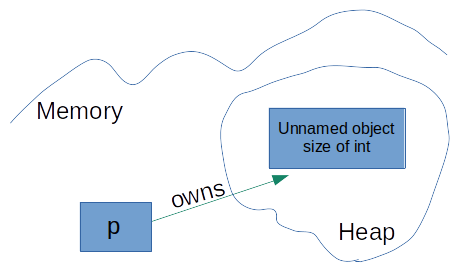
\includegraphics[width=1\textwidth, height=1\textheight, keepaspectratio]{./imgs/unique_ptr_definition.png}
	\caption{Unique ptr}
	\label{fig:unique_ptr_definition}
\end{figure}

\textsf{\small Se lo \textbf{unique\_ptr} viene distrutto, anche la memoria allocata nell'heap viene distrutta di conseguenza.} \\

\begin{figure}[H]
	\centering
	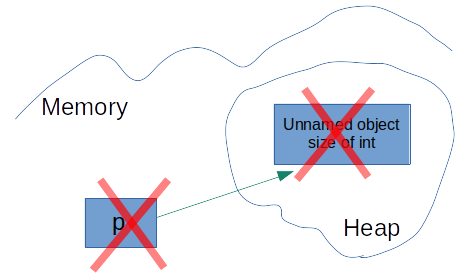
\includegraphics[width=1\textwidth, height=1\textheight, keepaspectratio]{./imgs/unique_ptr_delete.png}
	\caption{Unique ptr delete}
	\label{fig:unique_ptr_delete}
\end{figure}

\textsf{\small Per creare uno \textbf{unique\_ptr} si può anche utilizzare \textbf{std::make\_unique}.} \\

\begin{lstlisting}
	#include <iostream>
	
	class Rectangle {
		public:
			Rectangle(int w, int h)
			{
				this->width = w;
				this->height = h;
			}
		
			int area()
			{
				return width * height;
			}
		
		private:
			int width;
			int height;
	};

	int main()
	{
		auto pRect = std::make_unique<Rectangle>(3, 4);
		std::cout << "Area del rettangolo: " << pRect->area() << std::endl; //Output: Area del rettangolo: 12
		return 0;
	}
\end{lstlisting}

\subsubsection{Differenza tra std::make\_unique vs std::unique\_ptr}

\textsf{\small Ci sono varie ragioni per cui utilizzare \textbf{std::make\_unique} al posto di \textbf{std::unique\_ptr} con la new: } \\

\begin{itemize}
	\item \textsf{\small È sicuro nel caso si vogliano creare dei temporanei, mentre con la new ti devi ricordare la reogla: del non usare temporanei senza nome. } 
	\item \textsf{\small Con l'utilizzo di \textbf{make\_unique} si può finalmente evitare di usare la \textbf{new}, a differenza della vecchia regola: mai usare la \textbf{new} tranne per gli \textbf{unique\_ptr}.} 
	\item \textsf{\small Non richiede \emph{type usage} ridondante: \emph{unique\_ptr<T>(new T())} -> make\_unique<T>().} \\
	\item \textsf{\small Così da non dover esplicitare gli argomenti dei \emph{template types}.}
	\item \textsf{\small Aggiunge sicurezza riguardo le eccezioni.}
	\item \textsf{\small Altrimenti non potresti accedere al costruttore della classe fuori dallo \emph{scope} corrente.}
	%\item \textsf{\small }
\end{itemize}

\subsubsection{Ownership | move}

\textsf{\small Un \textbf{unique pointer} è una relazione 1 a 1 con l'oggetto allocato.} \\

\textsf{\small Non può essere copiato o passato per valore, però la \textbf{ownership} (proprietà) dell'oggetto può essere trasferita.} \\

\begin{lstlisting}
	#include <iostream>
	
	class Person {
		public:
			Person(std::string s) : name(s) {};
			~Person() { std::cout << "Libero spazio" << std::endl };
			
			std::string getName() { return this->name };
			
		private:
			std::string name;
	};

	int main()
	{
		auto ptrPerson = std::make_unique<Person>("Luigi");
		
		std::cout << "Nome: " << ptrPerson->getName() << std::endl; //Output: Nome: Luigi
		
		std::unique_ptr<Person> ptrPerson2;
		
		ptrPerson2 = std::move(ptrPerson);
		
		std::cout << "Nome: " << ptrPerson2->getName() << std::endl; //Output: Nome: Luigi
		
		std::cout << "Nome dopo il trasferimento dell'ownership: " << ptrPerson->getName() << std::endl; //Output: [non stampa niente]
		
		return 0;
	}
\end{lstlisting}

\begin{figure}[H]
	\centering
	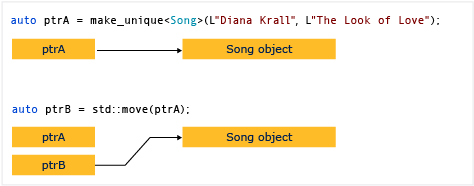
\includegraphics[width=1\textwidth, height=1\textheight, keepaspectratio]{./imgs/unique_ptr_move2.png}
	\caption{Unique ptr move}
	\label{fig:unique_ptr_move2}
\end{figure}

\subsubsection{Operazioni sugli unique\_ptr}

\textsf{\small Varie operazioni sono supportate sugli \textbf{unique\_ptr}: } \\

\begin{itemize}
	\item \textsf{\small \textbf{*} : Dereferenza del puntatore.}
	\item \textsf{\small \textbf{->} : Accedere ai membri della classe.}
	\item \textsf{\small \textbf{.get()} : per ottenere il \emph{raw pointer} del \textbf{unique\_ptr} (non cancellarlo, perché è gestito dal unique pointer; è da usare solo per calcoli).}
	\item \textsf{\small \textbf{.reset(new int())} : cancella il vecchio oggetto e ne crea uno nuovo (al posto di new int() avremmo potuto passare qualsiasi altro oggetto, era per fare un esempio).}
	\item \textsf{\small \textbf{move} : trasferisce la proprietà del \textbf{unique\_ptr}.}
	\item \textsf{\small \textbf{swap} : per scambiare due \textbf{unique pointers}.}
	\item \textsf{\small \textbf{if(unique\_ptr)} : se passiamo uno \textbf{unique\_ptr} all'if restituisce falso se non è associato a nessun oggetto.}
	%\item \textsf{\small \textbf{} : }
\end{itemize}

\subsubsection{Passare uno unique\_ptr ad una funzione}

\textsf{\small Utilizziamo \textbf{std::move} per trasferire la proprietà del \textbf{unique\_ptr}.} \\

\begin{lstlisting}
	#include <iostream>
	#include<memory>
	
	struct A {
		int x;
		~A() { std::cout << "Libero spazio" << std::endl };
	};

	void passUniquePtr(std::unique_ptr<A> a)
	{
		// Usciti dalla funzione lo unique\_ptr e il suo oggetto vengono cancellati, perché locali alla funzione.
		std::cout << "Puntatore ricevuto" << '\n';
		a->x = 5;
		std::cout << "a.x: " << a->x << std::endl;
	}

	int main()
	{
		auto ptrA = std::make_unique<A>();
		passUniquePtr(std::move(ptrA));
		
		// true = ptrA è vuoto.
		if(!ptrA)
		{
			std::cout << "ptrA è vuoto" << std::endl;
		}
	
		//Output: Puntatore ricevuto
		//Output: a.x: 5
		//Output: Libero spazio
		//Output: ptrA è vuoto
		return 0;
	}
\end{lstlisting} 

\subsubsection{Restituire un unique\_ptr}

\textsf{\small Si può restituire uno \textbf{unique\_ptr} da una funzione. } \\

\begin{lstlisting}
	#include <iostream>
	#include <memory>
	
	class A {};
	
	std::unique_ptr<A> returnUniquePtr()
	{
		auto a = std::make_unique<A>();
		return a;
	}

	int main()
	{
		auto ptrA = returnUniquePtr();
		
		if(ptrA)
		{
			std::cout << "ptrA ha un oggetto. " << std::endl;	
		}
	
		//Output: ptrA ha un oggetto.
		return 0;
	}
\end{lstlisting}

\subsubsection{Membri delle classi: unique pointer vs raw pointer vs reference}

\textsf{\small } \\

\begin{itemize}
	\item \textsf{\small \textbf{Unique pointer membro della classe} : la classe è la proprietaria dell'oggetto del puntatore.}
	\item \textsf{\small \textbf{Raw pointer membro della classe} : La classe è un osservatore e non è responsabile di rimuovere l'oggetto puntato dal puntatore. Viene rimosso da uno smart pointer fuori dalla classe.}
	\item \textsf{\small \textbf{Referenza membro della classe} : è garantito che la referenza contiene dati validi mentre la classe è "viva".}
	%\item \textsf{\small }
\end{itemize}

\subsection{share pointers}

\textsf{\small \textbf{Definizione: } Gli \textbf{shared pointers} sono un tipo di \textbf{smart pointers} dove più di un puntatore può puntare allo stesso oggetto e un contatore (\emph{Reference Counter}) verrà mantenuto di conseguenza.} \\

\textsf{\small Abbiamo sempre bisogno di includere l'header \textbf{<memory>} per poterlo utilizzare.} \break

\begin{lstlisting}
	#include <iostream>
	#include <memory>
	
	class A {
		public:
			int x;
			A(int x) : x(x){};
	};

	int main()
	{
		auto sharedPtr1 = std::make_shared<A>(7); // oppure si può anche fare: std::shared\_ptr<A> sharedPtr1(new A{7});
		
		std::shared_ptr<A> sharedPtr2 = sharedPtr1;
		std::shared_ptr<A> sharedPtr3 = sharedPtr1;
		
		// Tutti e tre gli \textbf{shared1\_ptr} puntano allo stesso oggetto.
		return 0;
	}
\end{lstlisting}

\begin{figure}[H]
	\centering
	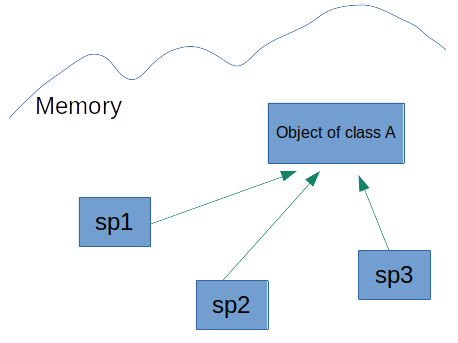
\includegraphics[width=1\textwidth, height=1\textheight, keepaspectratio]{./imgs/shared_ptr3.png}
	\caption{Shared ptr}
	\label{fig:shared_ptr3}
\end{figure}

\textsf{\small Possiamo creare uno \textbf{shared pointer} sia con \textbf{shared\_ptr} sia con \textbf{make\_shared}.} \\

\subsubsection{Differenza tra std::shared\_ptr vs std::make\_shared}

\textsf{\small Una delle differenze tra questi due è che \textbf{make\_shared} performa una sola allocazione nell'heap, mentre \textbf{shared\_ptr} ne fa due.} \\

\textsf{\small \textbf{shared\_ptr} si occupa di due entità: } \\

\begin{itemize}
	\item \textsf{\small Il blocco di controllo (\emph{control block}) che memorizza dei meta data come \emph{ref-counts} (contatore delle referenze all'oggetto), \emph{type-erased deleter}, ecc..}
	\item \textsf{\small l'oggetto stesso.}
\end{itemize}

\textsf{\small \textbf{std::make\_shared} fa una singola allocazione nell'heap per lo spazio necessario sia per il \emph{control block} sia per \emph{l'oggetto}. } \break

\textsf{\small Inoltre \textbf{std::make\_shared} è \emph{exception-safe} (sicuro per quanto riguarda le eccezioni).} \\

\textsf{\small Per di più, \textbf{make\_shared} sfrutta dell'ottimizzazione conosciuta come \emph{We know Where You Live} che permette al \emph{control block} di essere un piccolo puntatore, quindi \textbf{make\_shared} non solo evita un'ulteriore allocazione, ma alloca anche meno memoria totale.} \break

\textsf{\small Un problema che potrebbe esserci per quanto riguarda \textbf{std::make\_shared} è che visto che fa una singola allocazione, non c'è modo di deallocare la memoria del \emph{control block} e dell'\emph{oggetto} in modo indipendente. Un altro svantaggio, di conseguenza è che essendoci una singola allocazione, la memoria non può essere deallocata finché il \emph{control block} non è più usato. } \\

\subsubsection{Operazioni sui shared pointers}

\textsf{\small Sono possibili varie operazioni sugli \textbf{shared pointers}: } \\

\begin{itemize}
	\item \textsf{\small \textbf{(*nomepuntatore).variabile} : dereferenza}
	\item \textsf{\small \textbf{nomepuntatore->variabile} : dereferenza come sopra}
	\item \textsf{\small \textbf{.get()} : per poter accedere al \emph{raw pointer} chiamato \textbf{stored pointer}.}
	\item \textsf{\small \textbf{use\_count()} : per ottenere il numero di \textbf{shared\_ptr} che puntano allo stesso oggetto.}
	\item \textsf{\small \textbf{.reset()} : scollega e svuota il puntatore.}
\end{itemize}

\textsf{\small Lo \textbf{shared pointer} inoltre allo \emph{stored pointer}, possiede un secondo puntatore che punta ad un \textbf{control block}. Il \emph{control block} ha un \emph{reference counter} (contatore delle referenze) che memorizza il numero di \textbf{shared pointers} che puntano allo stesso oggetto.} \\

\begin{figure}[H]
	\centering
	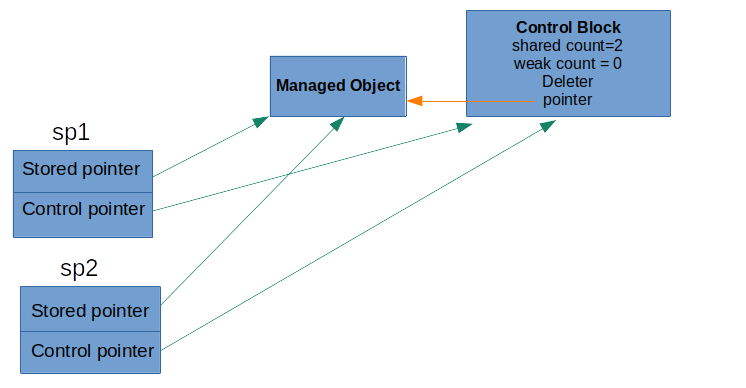
\includegraphics[width=1.2\textwidth, height=1.2\textheight, keepaspectratio]{./imgs/shared_ptr_structure.png}
	\caption{Shared ptr structure}
	\label{fig:shared_ptr_structure}
\end{figure}

\subsubsection{Distruzione degli shared pointers}

\textsf{\small Quando verrà eliminato l'oggetto gestito dagli \textbf{shared\_ptr}?} \\

\textsf{\small Quando uno \textbf{shared pointer} viene distrutto, allora il \emph{control block} decrementerà il \emph{reference counter}.} \\

\textsf{\small L'oggetto verrà eliminato quando l'ultimo \textbf{shared\_ptr} verrà eliminato.} \\

\begin{lstlisting}
	#include <iostream>
	#include <memory>
	
	class A {
		public:
			int x;
			A(int x) : x(x) {};
	};

	int main()
	{
		auto shrPtr1 = std::make_shared<A>(5);
		auto shrPtr2 = shrPtr1;
		auto shrPtr3 = shrPtr1;
		
		{
			auto shrPtr4 = shrPtr1;
			std::cout << shrPtr1.use_count() << std::endl; //Output: 4
		}
		
		std::cout << shrPtr1.use_count() << std::endl; //Output: 3
		
		shrPtr3 = std::make_shared<A>(8); // shrPtr3 punta ad un altro oggetto.x
		
		shrPtr2.reset(); // shrPtr2 scollegato e svuotato.
		
		std::cout << shrPtr1.use_count() << std::endl; //Output: 1
		return 0;
	}
\end{lstlisting}

\begin{figure}[H]
	\centering
	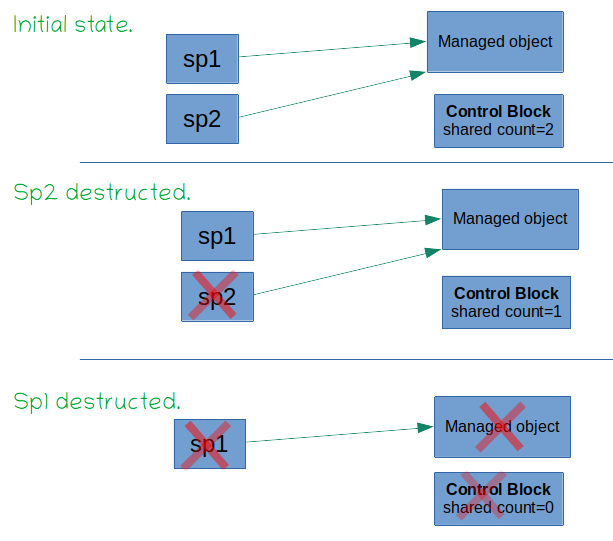
\includegraphics[width=1\textwidth, height=1\textheight, keepaspectratio]{./imgs/shared_ptr_destruction.png}
	\caption{Shared ptr destruction}
	\label{fig:shared_ptr_destruction}
\end{figure}

\subsubsection{Passare gli shared pointers ad una funzione}

\textsf{\small Se una funzione vuole l'\emph{ownership} (proprietà) su un \textbf{shared\_ptr}, possiamo passarlo per valore: } \\

\begin{lstlisting}
	#include <iostream>
	#include <memory>
	
	void function(std::shared_ptr<int> sp)
	{
		std::cout << sp.use_count() << std::endl;
	}

	int main()
	{
		auto sp1 = std::make_shared<int>(6);
		std::cout << sp1.use_count() << std::endl; //Output: 1
		
		function(sp1); //Output: 2
		
		std::cout << sp1.use_count() << std::endl; //Output: 1 (lo shared\_ptr nella funzione "function" viene distrutto una volta usciti da essa, perché è locale alla funzione)
		return 0;
	}
\end{lstlisting}

\subsubsection{Restituire gli shared pointers}

\textsf{\small Una funzione può restituire \textbf{shared\_ptr} per valore: } \\

\begin{lstlisting}
	#include <iostream>
	#include <memory>
	
	std::shared_ptr<int> function()
	{
		auto sp = std::make_shared<int>(9);
		return sp;
	}

	int main()
	{
		auto sp1 = function(); // Lo shared\_ptr dentro alla funzione non esiste più, però viene ritornato e recuperato nella variabile sp1.
		
		std::cout << sp1.use_count() << std::endl; //Output: 1
		std::cout << *sp1 << std::endl; //Output: 9
		return 0;
	}
\end{lstlisting}

\textsf{\small Un problema col restituire uno \textbf{shared\_ptr}, se lo devi restituire al "mondo esterno", meglio restituirlo come \emph{reference}, perché altrimenti uno potrebbe chiamare la \textbf{.reset()} su quello \textbf{shared pointer}.} \break

\textsf{\small Un altro modo per restituire uno \textbf{shared\_ptr} è attraverso \emph{std::allocate\_shared}.} \\

\begin{lstlisting}
	#include <iostream>
	#include <memory>
	
	int main () {
		std::allocator<int> alloc;    // allocatore di default per gli int.
		std::default_delete<int> del; // deleter di default per gli int.
		
		std::shared_ptr<int> foo = std::allocate_shared<int> (alloc,12);
		
		auto bar = std::allocate_shared<int> (alloc,24);
		
		auto baz = std::allocate_shared<std::pair<int,int>> (alloc,33,44);
		
		std::cout << "*foo: " << *foo << '\n'; //Output: *foo: 12
		std::cout << "*bar: " << *bar << '\n'; //Output: *bar: 24
		std::cout << "*baz: " << baz->first << ' ' << baz->second << '\n'; //Output: *baz: 33 44
		
		return 0;
	}
\end{lstlisting}

\subsubsection{static\_pointer\_cast}

\textsf{\small \textbf{Definizione: } \textbf{static\_pointer\_cast} è una funzione, non una keyword e restituisce uno \textbf{shared\_ptr} che possiede e contiene un puntatore all'oggetto costruito.} \\

\textsf{\small Se il parametro passato non è vuoto, ciò che viene restituito condivide la proprietà con il parametro passato, quindi il contatore viene incrementato di 1.} \\

\textsf{\small Se il parametro è vuoto (non possiede nulla), allora l'oggetto ritornato è uno \textbf{shared\_ptr} vuoto.} \\

\begin{lstlisting}
	#include <iostream>
	#include <memory>
	
	class Base {};
	
	class Derived : public Base {
		public:
			void print()
			{
				std::cout << "Hello World!" << std::endl;
			}
	};

	int main()
	{
		std::shared_ptr<Base> spBase(std::make_shared<Derived>());
		
		std::static_pointer_cast<Derived>(spBase)->print();
		
		static_cast<Derived*>(spBase.get())->print();
		
		//Output: Hello World!
		//Output: Hello World!
		return 0;
	}
\end{lstlisting}

\begin{figure}[H]
	\centering
	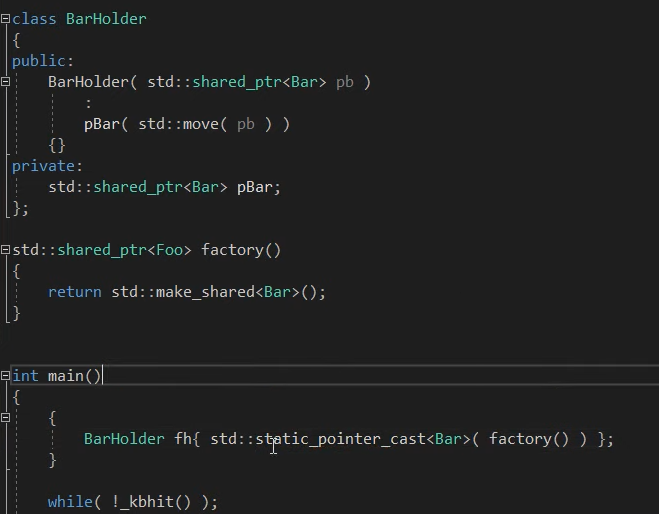
\includegraphics[width=1\textwidth, height=1\textheight, keepaspectratio]{./imgs/std_shared_ptr_std_static_pointer_cast2.png}
	\caption{Static pointer cast}
	\label{fig:std_shared_ptr_std_static_pointer_cast2}
\end{figure}

%TODO: dynamic_pointer_cast (volendo, ma non necessario, giusto per approfondimento)
%TODO: const_pointer_cast

\subsubsection{Performance degli shared pointers}

\textsf{\small Uno \textbf{shared pointer} ha bisogno di due \emph{raw pointers}. Un insieme di \textbf{shared pointers} hanno bisogno di essere gestiti da una \emph{control unit} (\emph{control block}). Quindi la memoria che uno \textbf{shared pointer} occupa è maggiore dei \emph{raw} e degli \textbf{unique} pointers.} \\

\subsubsection{Shared pointers, unique pointers or raw pointers}

\textsf{\small Se un oggetto ha bisogno di un singolo proprietario per tutta la durata del programma e possiamo immaginare il puntatore come un'entità singola, allora usiamo un \textbf{unique pointer}. Per delle performance più buone gli \textbf{unique pointers} sono migliori rispetto agli \textbf{shared pointers}.} \\

\textsf{\small Gli \textbf{shared pointers} sono utili dove non abbiamo bisogno di pensare alle \emph{performance}, \emph{ownership} e \emph{lifetime} degli oggetti.}

\subsection{weak pointers}

\textsf{\small \textbf{Definizione: } I \textbf{weak pointers} sono un tipo di \textbf{smart pointers} che non prende la proprietà dell'oggetto, ma agisce come un osservatore. Non partecipa al \emph{reference counter} (non viene contato) e non estende la \emph{lifetime} dell'oggetto. Sono usati, principalmente, per rompere la dipendenza circolare degli \textbf{shared pointers}.} \\

\subsubsection{Problema della dipendenza ciclica}

\textsf{\small \textbf{Definizione: } Mettiamo di avere due classi: A e B, se entrambe hanno un puntatore che punta all'altra, avremo un ciclo e il \emph{use\_count()} non arriverà mai a 0, il che crea un problema nella rimozione di questi due puntatori.} \\

\begin{figure}[H]
	\centering
	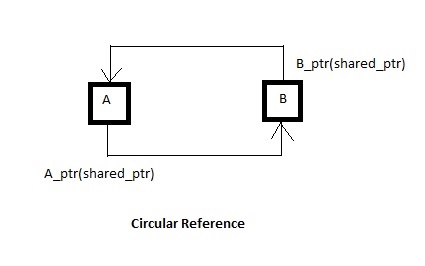
\includegraphics[width=1\textwidth, height=1\textheight, keepaspectratio]{./imgs/shared_ptr_problem_cyclic_dependency.jpg}
	\caption{Cyclic dependency}
	\label{fig:shared_ptr_problem_cyclic_dependency}
\end{figure}

\textsf{\small Per questo motivo usiamo gli \textbf{weak pointers}, perché non vengono conteggiati nel \emph{reference counter}. Possono, comunque avere accesso all'oggetto.} \\

\begin{figure}[H]
	\centering
	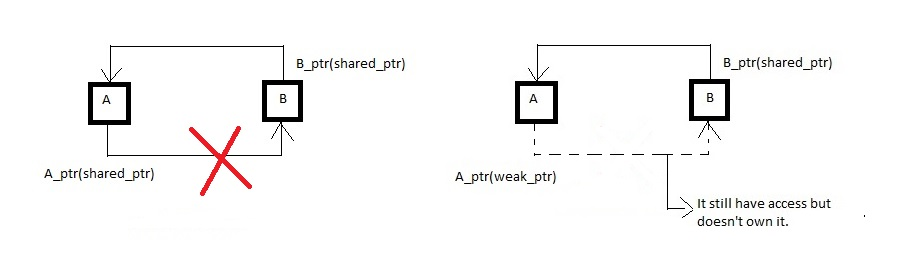
\includegraphics[width=1.2\textwidth, height=1.2\textheight, keepaspectratio]{./imgs/shared_ptr_problem_cyclic_dependency2.jpg}
	\caption{Cyclic dependency}
	\label{fig:shared_ptr_problem_cyclic_dependency2}
\end{figure}

\textsf{\small Quindi, il problema della \emph{dipendenza ciclica} si risolve con l'utilizzo degli \textbf{weak pointers}.} \\

\subsubsection{Quando usare i weak pointers?}

\textsf{\small \textbf{Quando usare i weak pointers?}} \break

\textsf{\small Quando vuoi riferire al tuo oggetto da molteplici posti, per quelle referenze dove non è okay ignorarle e deallocarle.} \\

%TODO: risolvere problema del danglin pointer

\subsubsection{Operazioni sugli weak pointers}

\textsf{\small Ci sono varie operazioni sui \textbf{weak pointers}: } \\

\begin{itemize}
	\item \textsf{\small \textbf{*} : dereferenza}
	\item \textsf{\small \textbf{->} : dereferenza, accedere ai membri della classe/struct, ecc..}
	\item \textsf{\small \textbf{.lock()} : restituisce uno \textbf{shared\_ptr} con le informazioni preservate nel \textbf{weak\_ptr} se non è \emph{expired}. Se il \textbf{weak\_ptr} è \emph{expired} (scaduto), la funzione restituisce un \textbf{shared\_ptr} vuoto.}
	%\item \textsf{\small \textbf{.get()} : }
	\item \textsf{\small \textbf{.reset()} : cancella il vecchio oggetto e ne crea uno nuovo.}
	\item \textsf{\small \textbf{.swap()} : scambia due \textbf{weak pointers}.}
	\item \textsf{\small \textbf{.use\_count()} : restituisce il numero di \textbf{shared pointers} che puntano allo stesso oggetto.}
	\item \textsf{\small \textbf{.expired()} : restituisce se il \textbf{weak\_ptr} è vuoto o non ci sono più \textbf{shared\_ptr} nel \emph{owner group}. I puntatori "scaduti" (\emph{expired}) sono come \textbf{weak pointers} vuoti quando \emph{locked}, e non possono quindi essere più usati.}
	\item \textsf{\small \textbf{.owner-before()} : restituisce se l'oggetto deve andare prima del parametro. Se l'oggetto appartiene allo stesso \emph{owner group} del parametro, allora restituisce \emph{false}, anche se il valore memorizzato dai puntatori è diverso.}
	%\item \textsf{\small \textbf{} : }
\end{itemize}

\begin{lstlisting}
	#include <iostream>
	#include <memory>
	
	class Person {
		public:
			std::string name;
			Person(std::string name) : name(name){};
	};
	
	int main()
	{
		std::weak_ptr<Person> wp;
		
		auto teacher = std::make_shared<Person>("Giorgio");
		
		wp = teacher;
		
		// Per controllare se l'oggetto è ancora lì o no.
		// lock() restituisce un shared\_ptr temporaneo.
		if(auto temp = wp.lock())
		{
			std::cout << temp->name << std::endl;
		} else {
			std::cout << "L'oggetto non c'è più" << std::endl;
		}
		return 0;
	}
\end{lstlisting}

\begin{figure}[H]
	\centering
	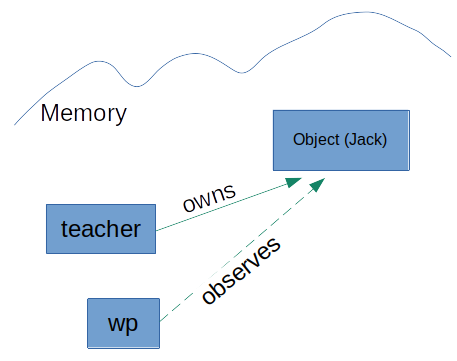
\includegraphics[width=1\textwidth, height=1\textheight, keepaspectratio]{./imgs/weak_ptr1.png}
	\caption{Weak pointers}
	\label{fig:weak_ptr1}
\end{figure}

\textsf{\small Uno \textbf{shared pointer} ha un \textbf{control block} che conta il numero di \textbf{shared pointers} e di \textbf{weak pointers}. Quando il contatore degli \textbf{shared pointers} arriva a 0, l'oggetto viene eliminato, ma il \emph{control block} resta vivo finché il contatore dei \textbf{weak pointers} non raggiunge 0.} \\

%TODO: altre subsections

% -------------------------- SECTION: UNIFORM REAL DISTRIBUTION ----------------------

\newpage

\section{Uniform Real Distribution}

\textsf{\small \textbf{Definizione: } } \\

%TODO: Dependency Injection

% -------------------------- SECTION: 7 CONCETTI AVANZATI ----------------------------

\newpage

%TODO: Questo come ultimo argomento del capitolo!

%TODO: Come prima cosa qui aggiungere quell'immagine sui 7 concetti avanzati.

%TODO: RAII, Return Type Resolver, Type Erasure, CRTP, Virtual Constructor, SFINAE, Proxy.

\section{7 Concetti Avanzati}

\subsection{RAII}

\textsf{\small \textbf{Definizione: } } \\ %TODO: scrivere che abbiamo già trattato questo argomento nel precedente capitolo oppure nel capitolo Concetti Intermedi, ma voglio comunque ripassarlo qui.

\subsection{Return Type Resolver}

\subsection{Type Erasure}

\subsection{CRTP}

\subsection{Virtual Constructor}

\subsection{SFINAE}

%TODO: tratterò questo argomento anche nel capitolo Le gemme della libreria degli Algoritmi.

\subsection{Proxy}

% ------------------------------------------------------------------------------------